\section{Quiver Mutation}

\begin{frame}{Adding the Quiver}
    We associate a \textbf{quiver} (directed multigraph) to the triangulation by placing vertices and arrows so that for each triangle there is a clockwise $3$-cycle between its edges:
    \begin{center}
		\begin{tikzpicture}[scale=0.3,baseline=(current bounding box.center)]
			% Hexagon Vertices
			\begin{scope}[every node/.style={circle,fill,draw,inner sep=2pt}]
				\node (A) at (5,0) {};
				\node (B) at (2.5,4.33) {};
				\node (C) at (-2.5,4.33) {};
				\node (D) at (-5,0) {};
				\node (E) at (-2.5,-4.33) {};
				\node (F) at (2.5,-4.33) {};
			\end{scope}
			
			% Edges
			\begin{scope}[>={Stealth[black]},
				every node/.style={fill=white,circle},
				every edge/.style={draw=black,thick}]
				
				% sides
				\path (A) edge (B);
				\path (B) edge (C);
				\path (C) edge (D);
				\path (D) edge (E);
				\path (E) edge (F);
				\path (F) edge (A);
			\end{scope}

			% Edges
			\begin{scope}[>={Stealth[blue]},
				every node/.style={fill=white,circle},
				every edge/.style={draw=blue,thick}]
				
				% diagonals
				\path (A) edge (C) edge (D) edge (E);
			\end{scope}

			% Quiver Vertices
			\begin{scope}[every node/.style={circle,fill=red,draw=red,inner sep=2pt}]
				\node (Q1) at (3.75,2.165) {};
				\node (Q2) at (0,4.33) {};
				\node (Q3) at (1.25,2.165) {};
				\node (Q4) at (0,0) {};
				\node (Q5) at (-3.75,2.165) {};
				\node (Q6) at (-3.75,-2.165) {};
				\node (Q7) at (0,-4.33) {};
				\node (Q8) at (3.75,-2.165) {};
				\node (Q9) at (1.25,-2.165) {};
			\end{scope}

			% Quiver arrows
			\begin{scope}[>={Stealth[red,inset=1pt,length=7pt]},
				every node/.style={fill=white,circle},
				every edge/.style={draw=red,thick}]
				
				\path [<-] (Q1) edge (Q2);
				\path [<-] (Q2) edge (Q3);
				\path [<-] (Q3) edge (Q1);

				\path [<-] (Q4) edge (Q3);
				\path [<-] (Q3) edge (Q5);
				\path [<-] (Q5) edge (Q4);

				\path [<-] (Q4) edge (Q6);
				\path [<-] (Q6) edge (Q9);
				\path [<-] (Q9) edge (Q4);

				\path [<-] (Q9) edge (Q7);
				\path [<-] (Q7) edge (Q8);
				\path [<-] (Q8) edge (Q9);
			\end{scope}
		\end{tikzpicture}
		\begin{tikzpicture}[baseline=(current bounding box.center)]
			\begin{scope}[>={Stealth[black,inset=1pt,length=10pt]},
				every edge/.style={draw=black,thick}]
				
				\node (A) at (0,0) {};
				\node (B) at (1.5,0) {};
				\path[<->] (A) edge (B);
			\end{scope}
		\end{tikzpicture}
		\begin{tikzpicture}[scale=0.3,baseline=(current bounding box.center)]
			% Hexagon Vertices
			\begin{scope}[every node/.style={circle,fill,draw,inner sep=2pt}]
				\node (A) at (5,0) {};
				\node (B) at (2.5,4.33) {};
				\node (C) at (-2.5,4.33) {};
				\node (D) at (-5,0) {};
				\node (E) at (-2.5,-4.33) {};
				\node (F) at (2.5,-4.33) {};
			\end{scope}
			
			% Edges
			\begin{scope}[>={Stealth[black]},
				every node/.style={fill=white,circle},
				every edge/.style={draw=black,thick}]
				
				% sides
				\path (A) edge (B);
				\path (B) edge (C);
				\path (C) edge (D);
				\path (D) edge (E);
				\path (E) edge (F);
				\path (F) edge (A);
			\end{scope}

			% Edges
			\begin{scope}[>={Stealth[blue]},
				every node/.style={fill=white,circle},
				every edge/.style={draw=blue,thick}]
				
				% diagonals
				\path (A) edge (D) edge (E);
				\path (D) edge (B);
			\end{scope}

			% Quiver Vertices
			\begin{scope}[every node/.style={circle,fill=red,draw=red,inner sep=2pt}]
				\node (Q1) at (3.75,2.165) {};
				\node (Q2) at (0,4.33) {};
				\node (Q3) at (-1.25,2.165) {};
				\node (Q4) at (0,0) {};
				\node (Q5) at (-3.75,2.165) {};
				\node (Q6) at (-3.75,-2.165) {};
				\node (Q7) at (0,-4.33) {};
				\node (Q8) at (3.75,-2.165) {};
				\node (Q9) at (1.25,-2.165) {};
			\end{scope}

			% Quiver arrows
			\begin{scope}[>={Stealth[red,inset=1pt,length=7pt]},
				every node/.style={fill=white,circle},
				every edge/.style={draw=red,thick}]
				
				\path [<-] (Q1) edge (Q3);
				\path [<-] (Q3) edge (Q4);
				\path [<-] (Q4) edge (Q1);

				\path [<-] (Q3) edge (Q2);
				\path [<-] (Q2) edge (Q5);
				\path [<-] (Q5) edge (Q3);

				\path [<-] (Q4) edge (Q6);
				\path [<-] (Q6) edge (Q9);
				\path [<-] (Q9) edge (Q4);

				\path [<-] (Q9) edge (Q7);
				\path [<-] (Q7) edge (Q8);
				\path [<-] (Q8) edge (Q9);
			\end{scope}
		\end{tikzpicture}
	\end{center}
    Notice that the two triagulations differ only in the top half of the hexagon (i.e. effects of flip on quiver are ``local'')
\end{frame}

\begin{frame}{Adding the Quiver (cont.)}
    \begin{definition}
		\justifying		
        A \textbf{quiver} $Q = (Q_0, Q_1, s, t)$ where $Q_0$ is vertex set, $Q_1$ is the arrow set, $s:Q_1 \to Q_0$ gives the source vertex of an arrow, $t:Q_1 \to Q_0$ gives the target vertex of an arrow.
    \end{definition}
	\begin{center}
        \begin{tikzpicture}[scale=0.25,baseline=(current bounding box.center)]
			% Hexagon Vertices
			\begin{scope}[every node/.style={circle,fill,draw,inner sep=2pt}]
				\node (A) at (5,0) {};
				\node (B) at (2.5,4.33) {};
				\node (C) at (-2.5,4.33) {};
				\node (D) at (-5,0) {};
				\node (E) at (-2.5,-4.33) {};
				\node (F) at (2.5,-4.33) {};
			\end{scope}
			
			% Edges
			\begin{scope}[>={Stealth[black]},
				every node/.style={fill=white,circle},
				every edge/.style={draw=black,thick}]
				
				% sides
				\path (A) edge (B);
				\path (B) edge (C);
				\path (C) edge (D);
				\path (D) edge (E);
				\path (E) edge (F);
				\path (F) edge (A);
			\end{scope}

			% Edges
			\begin{scope}[>={Stealth[blue]},
				every node/.style={fill=white,circle},
				every edge/.style={draw=blue,thick}]
				
				% diagonals
				\path (A) edge (C) edge (D) edge (E);
			\end{scope}

			% Quiver Vertices
			\begin{scope}[every node/.style={circle,fill=red,draw=red,inner sep=2pt}]
				\node (Q1) at (3.75,2.165) {};
				\node (Q2) at (0,4.33) {};
				\node (Q3) at (1.25,2.165) {};
				\node (Q4) at (0,0) {};
				\node (Q5) at (-3.75,2.165) {};
				\node (Q6) at (-3.75,-2.165) {};
				\node (Q7) at (0,-4.33) {};
				\node (Q8) at (3.75,-2.165) {};
				\node (Q9) at (1.25,-2.165) {};
			\end{scope}

			% Quiver arrows
			\begin{scope}[>={Stealth[red,inset=1pt,length=7pt]},
				every node/.style={fill=white,circle},
				every edge/.style={draw=red,thick}]
				
				\path [<-] (Q1) edge (Q2);
				\path [<-] (Q2) edge (Q3);
				\path [<-] (Q3) edge (Q1);

				\path [<-] (Q4) edge (Q3);
				\path [<-] (Q3) edge (Q5);
				\path [<-] (Q5) edge (Q4);

				\path [<-] (Q4) edge (Q6);
				\path [<-] (Q6) edge (Q9);
				\path [<-] (Q9) edge (Q4);

				\path [<-] (Q9) edge (Q7);
				\path [<-] (Q7) edge (Q8);
				\path [<-] (Q8) edge (Q9);
			\end{scope}
		\end{tikzpicture}
    \end{center}
	\begin{definition}
        A \textbf{cluster quiver} is a quiver without $2$-cycles and loops.
    \end{definition}
    % \begin{enumerate}
    %     \item Quivers beneficial because easy to visualize cluster algebras corresponding to antisymmetric matrices with integer entries
    %     \begin{itemize}
    %         \item Obtained by labeling vertices by $[n] \coloneq \{1, 2, \ldots, n\}$ and placing $(a_{ij})$ arrows $i \to j$ if $(a_{ij})$ is positive
    %     \end{itemize}

    %     \item Connections to various topics in theoretical physics (e.g. Seiberg duality)
    % \end{enumerate}
\end{frame}

\begin{frame}{Generalizing Flips with Quiver Mutation}
    \textbf{Quiver mutation} at vertex $x$ of cluster quiver $Q$ gives new quiver $\mu_x(Q)$:
    \begin{enumerate}
        \item For each path $v \to x \to w$, add a new arrow $v \to w$
        \item Reverse orientation of arrows incident to $x$
        \item Remove any pairs of arrows forming $2$-cycles. Repeat until no more $2$-cycles are left
    \end{enumerate}

    Demonstrate on the top half of the triangulation from last slide by mutating the center vertex of the quiver:
    \begin{center}
        \begin{tikzpicture}[scale=0.3,baseline=(current bounding box.center)]
			% Hexagon Vertices
			\begin{scope}[every node/.style={circle,fill,draw,inner sep=2pt}]
				\node (A) at (5,0) {};
				\node (B) at (2.5,4.33) {};
				\node (C) at (-2.5,4.33) {};
				\node (D) at (-5,0) {};
			\end{scope}
			
			% Edges
			\begin{scope}[>={Stealth[black]},
				every node/.style={fill=white,circle},
				every edge/.style={draw=black,thick}]
				
				% sides
				\path (A) edge (B);
				\path (B) edge (C);
				\path (C) edge (D);
			\end{scope}

			% Edges
			\begin{scope}[>={Stealth[blue]},
				every node/.style={fill=white,circle},
				every edge/.style={draw=blue,thick}]
				
				% diagonals
				\path (A) edge (C) edge (D);
			\end{scope}

			% Quiver Vertices
			\begin{scope}[every node/.style={circle,fill=red,draw=red,inner sep=2pt}]
				\node (Q1) at (3.75,2.165) {};
				\node (Q2) at (0,4.33) {};
				\node (Q3) at (1.25,2.165) {};
				\node (Q4) at (0,0) {};
				\node (Q5) at (-3.75,2.165) {};
			\end{scope}

			% Label for center vertex
			\begin{scope}[every node/.style={inner sep=1pt}]
				\node (X) at (1.35,1.40) {$\color{red}x$};
			\end{scope}

			% Quiver arrows
			\begin{scope}[>={Stealth[red,inset=1pt,length=7pt]},
				every node/.style={fill=white,circle},
				every edge/.style={draw=red,thick}]
				
				\path [<-] (Q1) edge (Q2);
				\path [<-] (Q2) edge (Q3);
				\path [<-] (Q3) edge (Q1);

				\path [<-] (Q4) edge (Q3);
				\path [<-] (Q3) edge (Q5);
				\path [<-] (Q5) edge (Q4);
			\end{scope}
		\end{tikzpicture}
    \end{center}
\end{frame}

\begin{frame}{Example of Quiver Mutation}
    \begin{enumerate}
        \item[1.] For each path $v \to x \to w$, add a new arrow $v \to w$.
    \end{enumerate}
    \begin{center}
        \begin{tikzpicture}[scale=0.65,baseline=(current bounding box.center)]
			% Hexagon Vertices
			\begin{scope}[every node/.style={circle,fill,draw,inner sep=2pt}]
				\node (A) at (5,0) {};
				\node (B) at (2.5,4.33) {};
				\node (C) at (-2.5,4.33) {};
				\node (D) at (-5,0) {};
			\end{scope}
			
			% Edges
			\begin{scope}[>={Stealth[black]},
				every node/.style={fill=white,circle},
				every edge/.style={draw=black,thick}]
				
				% sides
				\path (A) edge (B);
				\path (B) edge (C);
				\path (C) edge (D);
			\end{scope}

			% Edges
			\begin{scope}[>={Stealth[blue]},
				every node/.style={fill=white,circle},
				every edge/.style={draw=blue,thick}]
				
				% diagonals
				\path (A) edge (C) edge (D);
			\end{scope}

			% Quiver Vertices
			\begin{scope}[every node/.style={circle,fill=red,draw=red,inner sep=2pt}]
				\node (Q1) at (3.75,2.165) {};
				\node (Q2) at (0,4.33) {};
				\node (Q3) at (1.25,2.165) {};
				\node (Q4) at (0,0) {};
				\node (Q5) at (-3.75,2.165) {};
			\end{scope}

			% Label for center vertex
			\begin{scope}[every node/.style={inner sep=1pt}]
				\node (X) at (1.35,1.70) {$\color{red}x$};
			\end{scope}

			% Quiver arrows
			\begin{scope}[>={Stealth[red,inset=1pt,length=7pt]},
				every node/.style={fill=white,circle},
				every edge/.style={draw=red,thick}]
				
				\path [<-] (Q1) edge[bend left=0] (Q2);
				\path [<-] (Q2) edge (Q3);
				\path [<-] (Q3) edge (Q1);

				\path [<-] (Q4) edge (Q3);
				\path [<-] (Q3) edge (Q5);
				\path [<-] (Q5) edge[bend left=0] (Q4);
			\end{scope}

            % Quiver arrows
			\begin{scope}[>={Stealth[red,inset=1pt,length=7pt]},
				every node/.style={fill=white,circle},
				every edge/.style={draw=red,thick,dashed}]
				
                \path[->] (Q1) edge[bend left=10] (Q4);
                \path[->] (Q1) edge[bend right=30] (Q2);
                \path[->] (Q5) edge (Q2);
                \path [->] (Q5) edge[bend right=30] (Q4);
			\end{scope}
		\end{tikzpicture}
    \end{center}
\end{frame}

\begin{frame}{Example of Quiver Mutation (cont.)}
    \begin{enumerate}
        \item[2.] Reverse orientation of arrows incident to $x$
    \end{enumerate}
    \begin{center}
        \begin{tikzpicture}[scale=0.65,baseline=(current bounding box.center)]
			% Hexagon Vertices
			\begin{scope}[every node/.style={circle,fill,draw,inner sep=2pt}]
				\node (A) at (5,0) {};
				\node (B) at (2.5,4.33) {};
				\node (C) at (-2.5,4.33) {};
				\node (D) at (-5,0) {};
			\end{scope}
			
			% Edges
			\begin{scope}[>={Stealth[black]},
				every node/.style={fill=white,circle},
				every edge/.style={draw=black,thick}]
				
				% sides
				\path (A) edge (B);
				\path (B) edge (C);
				\path (C) edge (D);
			\end{scope}

			% Edges
			\begin{scope}[>={Stealth[blue]},
				every node/.style={fill=white,circle},
				every edge/.style={draw=blue,thick}]
				
				% diagonals
				\path (A) edge (C) edge (D);
			\end{scope}

			% Quiver Vertices
			\begin{scope}[every node/.style={circle,fill=red,draw=red,inner sep=2pt}]
				\node (Q1) at (3.75,2.165) {};
				\node (Q2) at (0,4.33) {};
				\node (Q3) at (1.25,2.165) {};
				\node (Q4) at (0,0) {};
				\node (Q5) at (-3.75,2.165) {};
			\end{scope}

			% Label for center vertex
			\begin{scope}[every node/.style={inner sep=1pt}]
				\node (X) at (1.35,1.70) {$\color{red}x$};
			\end{scope}

			% Quiver arrows
			\begin{scope}[>={Stealth[red,inset=1pt,length=7pt]},
				every node/.style={fill=white,circle},
				every edge/.style={draw=red,thick}]
				
				\path [<-] (Q1) edge[bend left=0] (Q2);
				\path [<-] (Q5) edge[bend left=0] (Q4);

                \path[->] (Q1) edge[bend left=10] (Q4);
                \path[->] (Q1) edge[bend right=30] (Q2);
                \path[->] (Q5) edge (Q2);
                \path [->] (Q5) edge[bend right=30] (Q4);
			\end{scope}

            % Quiver arrows
			\begin{scope}[>={Stealth[red,inset=1pt,length=7pt]},
				every node/.style={fill=white,circle},
				every edge/.style={draw=red,thick,dashed}]
                
                \path [->] (Q2) edge (Q3);
				\path [->] (Q3) edge (Q1);

				\path [->] (Q4) edge (Q3);
				\path [->] (Q3) edge (Q5);
			\end{scope}
		\end{tikzpicture}
    \end{center}
\end{frame}

\begin{frame}{Example of Quiver Mutation (still cont.)}
    \begin{enumerate}
        \item[3.] Remove any pairs of arrows forming $2$-cycles. Repeat until no more $2$-cycles left
    \end{enumerate}
    \begin{center}
        \begin{tikzpicture}[scale=0.65,baseline=(current bounding box.center)]
			% Hexagon Vertices
			\begin{scope}[every node/.style={circle,fill,draw,inner sep=2pt}]
				\node (A) at (5,0) {};
				\node (B) at (2.5,4.33) {};
				\node (C) at (-2.5,4.33) {};
				\node (D) at (-5,0) {};
			\end{scope}
			
			% Edges
			\begin{scope}[>={Stealth[black]},
				every node/.style={fill=white,circle},
				every edge/.style={draw=black,thick}]
				
				% sides
				\path (A) edge (B);
				\path (B) edge (C);
				\path (C) edge (D);
			\end{scope}

			% Edges
			\begin{scope}[>={Stealth[blue]},
				every node/.style={fill=white,circle},
				every edge/.style={draw=blue,thick}]
				
				% diagonals
				\path (A) edge (C) edge (D);
			\end{scope}

			% Quiver Vertices
			\begin{scope}[every node/.style={circle,fill=red,draw=red,inner sep=2pt}]
				\node (Q1) at (3.75,2.165) {};
				\node (Q2) at (0,4.33) {};
				\node (Q3) at (1.25,2.165) {};
				\node (Q4) at (0,0) {};
				\node (Q5) at (-3.75,2.165) {};
			\end{scope}

			% Label for center vertex
			\begin{scope}[every node/.style={inner sep=1pt}]
				\node (X) at (1.35,1.70) {$\color{red}x$};
			\end{scope}

			% Quiver arrows
			\begin{scope}[>={Stealth[red,inset=1pt,length=7pt]},
				every node/.style={fill=white,circle},
				every edge/.style={draw=red,thick}]

                \path[->] (Q1) edge (Q4);
                \path[->] (Q5) edge (Q2);

                \path [->] (Q2) edge (Q3);
				\path [->] (Q3) edge (Q1);

				\path [->] (Q4) edge (Q3);
				\path [->] (Q3) edge (Q5);
			\end{scope}
		\end{tikzpicture}
    \end{center}
\end{frame}

\begin{frame}{Example of Quiver Mutation (still cont.)}
    Also update triangulation so it's consistent with quiver:
    \begin{center}
        \begin{tikzpicture}[scale=0.65,baseline=(current bounding box.center)]
			% Hexagon Vertices
			\begin{scope}[every node/.style={circle,fill,draw,inner sep=2pt}]
				\node (A) at (5,0) {};
				\node (B) at (2.5,4.33) {};
				\node (C) at (-2.5,4.33) {};
				\node (D) at (-5,0) {};
			\end{scope}
			
			% Edges
			\begin{scope}[>={Stealth[black]},
				every node/.style={fill=white,circle},
				every edge/.style={draw=black,thick}]
				
				% sides
				\path (A) edge (B);
				\path (B) edge (C);
				\path (C) edge (D);
			\end{scope}

			% Edges
			\begin{scope}[>={Stealth[blue]},
				every node/.style={fill=white,circle},
				every edge/.style={draw=blue,thick}]
				
				% diagonals
				\path (A) edge (D);
				\path (D) edge (B);
			\end{scope}

			% Quiver Vertices
			\begin{scope}[every node/.style={circle,fill=red,draw=red,inner sep=2pt}]
				\node (Q1) at (3.75,2.165) {};
				\node (Q2) at (0,4.33) {};
				\node (Q3) at (-1.25,2.165) {};
				\node (Q4) at (0,0) {};
				\node (Q5) at (-3.75,2.165) {};
			\end{scope}

			% Label for center vertex
			\begin{scope}[every node/.style={inner sep=1pt}]
				\node (X) at (-1.40,1.70) {$\color{red}x$};
			\end{scope}

			% Quiver arrows
			\begin{scope}[>={Stealth[red,inset=1pt,length=7pt]},
				every node/.style={fill=white,circle},
				every edge/.style={draw=red,thick}]
				
				\path [<-] (Q1) edge (Q3);
				\path [<-] (Q3) edge (Q4);
				\path [<-] (Q4) edge (Q1);

				\path [<-] (Q3) edge (Q2);
				\path [<-] (Q2) edge (Q5);
				\path [<-] (Q5) edge (Q3);
			\end{scope}
		\end{tikzpicture}
    \end{center}
    Flips of triangulation induce quiver mutation in associated quiver
\end{frame}

\begin{frame}{Play with Quiver Mutations Live}
    Dr. Bernhard Keller has a quiver mutation program \cite{mutationapp} on his website that you can play with:
    \begin{center}
        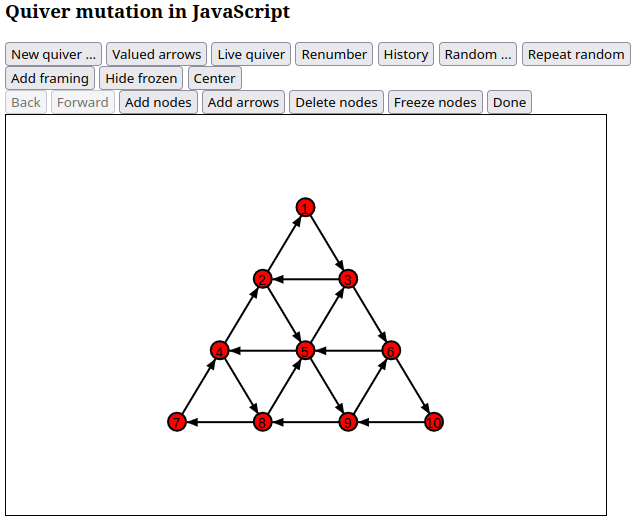
\includegraphics[scale=0.3]{figures/bkeller_app.png}
    \end{center}
	Google \textbf{``Keller Mutation App''}
\end{frame}

% \begin{frame}{Play with Quiver Mutations Live (cont.)}
%     Can be found by Googling ``\textbf{Keller Mutation App}''. Here is a QR code as well:
%     \begin{center}
%         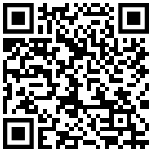
\includegraphics[scale=0.7]{figures/bkeller_qr.png}

%         \url{https://webusers.imj-prg.fr/~bernhard.keller/quivermutation/}
%     \end{center}
% \end{frame}

\begin{frame}{Properties of Quiver Mutation}
    \begin{enumerate}
        \item Quiver mutation is involutive: $\mu_A(\mu_A(Q)) = Q$
        \begin{center}
            \begin{tikzpicture}[scale=0.3,baseline=(current bounding box.center)]
                % Vertices
                \begin{scope}[every node/.style={circle,thick,draw,inner sep=1pt}]
                    \node (A) at (0,0) {$A$};
                    \node (B) at (0,5) {$B$};
                    \node (C) at (5,5) {$C$};
                    \node (D) at (5,0) {$D$};
                \end{scope}
                
                % Edges
                \begin{scope}[>={Stealth[black,inset=1pt,length=7pt]},
                    every node/.style={fill=white,circle},
                    every edge/.style={draw=black,thick}]
                    
                    \path [->] (D) edge (A);
                    \path [->] (A) edge (B);
                    \path [->] (B) edge[bend left=20] (D);
                    \path [->] (C) edge (B);
                    \path [->] (C) edge (D);
                \end{scope}
            \end{tikzpicture}
            \begin{tikzpicture}[baseline=(current bounding box.center)]
                \begin{scope}[>={Stealth[black,inset=1pt,length=7pt]},
                    every edge/.style={draw=black,thick},
                    every node/.style={fill=white,circle,inner sep=1pt}]
                    
                    \node (A) at (0,0) {};
                    \node (B) at (1.5,0) {};
                    \path[->] (A) edge node {$\mu_A$} (B);
                \end{scope}
            \end{tikzpicture}
            \begin{tikzpicture}[scale=0.3,baseline=(current bounding box.center)]
                % Vertices
                \begin{scope}[every node/.style={circle,thick,draw,inner sep=1pt}]
                    \node (A) at (0,0) {$A$};
                    \node (B) at (0,5) {$B$};
                    \node (C) at (5,5) {$C$};
                    \node (D) at (5,0) {$D$};
                \end{scope}
                
                % Edges
                \begin{scope}[>={Stealth[black,inset=1pt,length=7pt]},
                    every node/.style={fill=white,circle},
                    every edge/.style={draw=black,thick}]
                    
                    \path [->] (C) edge (B);
                    \path [->] (C) edge (D);
                    \path [->] (B) edge (A);
                    \path [->] (A) edge (D);
                \end{scope}
            \end{tikzpicture}
            \begin{tikzpicture}[baseline=(current bounding box.center)]
                \begin{scope}[>={Stealth[black,inset=1pt,length=7pt]},
                    every edge/.style={draw=black,thick},
                    every node/.style={fill=white,circle,inner sep=1pt}]
                    
                    \node (A) at (0,0) {};
                    \node (B) at (1.5,0) {};
                    \path[->] (A) edge node {$\mu_A$} (B);
                \end{scope}
            \end{tikzpicture}
            \begin{tikzpicture}[scale=0.3,baseline=(current bounding box.center)]
                % Vertices
                \begin{scope}[every node/.style={circle,thick,draw,inner sep=1pt}]
                    \node (A) at (0,0) {$A$};
                    \node (B) at (0,5) {$B$};
                    \node (C) at (5,5) {$C$};
                    \node (D) at (5,0) {$D$};
                \end{scope}
                
                % Edges
                \begin{scope}[>={Stealth[black,inset=1pt,length=7pt]},
                    every node/.style={fill=white,circle},
                    every edge/.style={draw=black,thick}]
                    
                    \path [->] (D) edge (A);
                    \path [->] (A) edge (B);
                    \path [->] (B) edge[bend left=20] (D);
                    \path [->] (C) edge (B);
                    \path [->] (C) edge (D);
                \end{scope}
            \end{tikzpicture}
        \end{center}
        
        \vfill 

        \item Number of vertices of quiver invariant under mutation
    \end{enumerate}
\end{frame}